%%%%%%%%%%%%%%%%%%%%%%%%%%%%%%%%%%%%%%%%%%%%%%%%%%%%%%
\section{Single-channel scattering: the optical model}
%%%%%%%%%%%%%%%%%%%%%%%%%%%%%%%%%%%%%%%%%%%%%%%%%%%%%%
\subsection{Optical model formalism}

\slide{Single-channel scattering: optical model potential}

\begin{itemize} 
\item {\red P} space represents just the ground state of projectile and target 
\item Wavefunction:
$$ \Psi = \underbrace{\Psi_P}_{\textrm{elastic}} + \underbrace{\Psi_Q}_{\textrm{non-elastic}} $$


\item Schrodinger equation in modelspace:
$$
\psframebox[fillcolor=magenta!5,linecolor=red,framearc=0.1,fillstyle=solid,framesep=5pt]{
 \left [T + H_\alpha (\xi_\alpha) + \rnode{F1}{ {\cal V} }  \right ] \Psi_P = E \Psi_P 
% \left [T + H_\alpha (\xi_\alpha) + \rnode{F1}{ \cal V} }  \right ] \Psi_P = E \Psi_P 
}%psframe
$$


$$
\rnode{T2}{
\psframebox[fillcolor=magenta!5,linecolor=red,framearc=0.1,fillstyle=solid,framesep=5pt]{
\rnode{T1}{ {\cal V} }=  \underbrace{ V_{PP} }_{ \textrm{Bare interaction}  } 
% {\cal V} =  \underbrace{ V_{PP} }_{ \textrm{Bare interaction}  } 
           +\underbrace{ V_{PQ} \frac{1}{E- H_{QQ} + i \epsilon} V_{QP} }_{  \textrm{``Polarization'' potential} } 
\equiv V_\mathrm{bare} + V_\mathrm{pol}
}%psframe
}%node
$$

\item ${\cal V} $ too complicated $\Rightarrow$ usually replaced by some phenomenological (complex) potential \textcolor{blue}{$U(\bR)$}  

\end{itemize}

{\nccurve[linecolor=blue,angleA=-90,angleB=90]{->}{F1}{T1}}

\end{frame}





%-------------------------------------------------
\slide{Microscopic folding model for ${\cal V}$  }
%-------------------------------------------------

Start from some (effective) nucleon-nucleon potential $v_{NN}$ (JLM, M3Y, etc):


\begin{enumerate}
\gitem{Single-folding potential:}

\begin{columns}
\column{0.6\textwidth}
$$
V(\bR) = \int \rho_t(\bs_t) v_{NN}(|\bR - \bs|) d\bs
$$
\hspace{1cm} \ding{43} $\rho_t(\bs_t)$=target g.s.~density.

\column{0.4\textwidth}
 \begin{center}\includegraphics[width=0.65\columnwidth]{figs/singlefold.eps}\end{center}
\end{columns}

\gitem{Double-folding potential:}
\begin{columns}
\column{0.6\textwidth}
$$
V(\bR) = \int \rho_p(\bs_p) \rho_t(\bs_t) v_{NN}(|\bR +\bs_p- \bs_t|) d\bs_p d\bs_t
$$
%\item[\ding{233}] $\rho(s)$=g.s.~density of target.

\column{0.4\textwidth}
 \begin{center}\includegraphics[width=0.65\columnwidth]{figs/doublefold.eps}\end{center}
\end{columns}
\end{enumerate}

\psframebox[fillcolor=blue!10,fillstyle=solid,framearc=0.2,framesep=2pt]{
\parbox{0.95\columnwidth}{%
\small
\bi
\item[\ding{233}] If $\rho_p$ and $\rho_t$ are g.s.\ densities, $V(\bR)$ accounts only for the bare potential ($V_{PP}$) (P-space part) and ignores the effect of non-elastic channels.
\item[\ding{233}] A model for $V_\mathrm{pol}$ must be supplied.
\item[\ding{233}] If  $v_{NN}$ is real, $V(\bR)$ is also real.
\ei
}}

\end{frame}


% ---------------------------------------------------------------------------
\slide{Phenomenological optical model}

{\brick Effective potential:} ${\cal V} \approx U(R)= U_\mathrm{nuc}(R) +  U_\mathrm{coul}(R) $

%\bigskip


\begin{itemize}
 \setlength{\itemsep}{10pt}
\item {\blue Coulomb potential:} charge sphere distribution

\begin{displaymath}
\psframebox[fillcolor=yellow,linecolor=red,framearc=0.1]{
U_\mathrm{coul}(R)=\left\{ \begin{array}{ll}
\frac{Z_1 Z_2 e^2}{2 R_c} \left( 3- \frac{R^2}{R_c^2}\right) & \textrm{if $R \leq R_c$} \\
\frac{Z_1 Z_2 e^2}{R}  & \textrm{if $R \geq R_c$} 
\end{array} \right .
}%psframebox
\end{displaymath}

\item {\blue Nuclear potential (complex):} Eg.~Woods-Saxon parametrization

\begin{equation}
\nonumber
\psframebox[fillcolor=yellow,linecolor=red,framearc=0.1]{
U_\mathrm{nuc}(R)=V(r) + i W(r) = -\frac{V_0}{1+\exp\left(\frac{R-R_0}{a_0}\right)}- i~\frac{W_0}{1+\exp\left(\frac{R-R_i}{a_i}\right)}
}%psframebox
\end{equation}

\ding{233} Popular parametrization: $R_0= r_0 (A_p^{1/3} + A_t^{1/3})$ \quad ($r_0$=reduced radius)

\medskip

\ding{233} For ``normal'' nuclei:  
\begin{itemize}
\item $r_0 \approx r_0  \sim 1.1-1.4$~fm
\item $a_0 \approx a_i \sim 0.5-0.7$~fm
\end{itemize}


\end{itemize}
\end{frame}
%----------------------------------------------------------------------------




% -------------------------------------------------------------------------
\slide{Elastic scattering within the optical model}
%\textcolor{blue}{How does one describe the motion of a particle in quantum mechanics?}

\begin{itemize}
\setlength{\itemsep}{12pt}
\item {\verde Effective Hamiltonian}: $$H = T_{\bR} + H_\alpha(\xi_\alpha) + U(\bR) \quad \quad (U(\bR)~ \textrm{complex!}) $$

\item {\verde $U(\bR)$ independent of $\{ \xi_\alpha \}$ } % $\Rightarrow$ $\Psi^{(+)}_{\bK}(\bR,\xi_\alpha)= $\chi^{}  
$$
\Psi^{(+)}_{\bK}(\xi_\alpha,\bR) = \Phi_{0}(\xi_\alpha) \chi^{(+)}_{0}(\bK,\bR)
$$

%\item[] {\blue $U(R)$}: optical model $\Rightarrow$ effective projectile-target interaction

%\begin{equation}
%H = T(\vec r) + U(r) 
%\nolabel
%\end{equation} 
%\item {\verde Schr\"odinger equation}: $[H-E]\Psi^{+}_{\bK}(\bR)=0$
\item {\verde Schr\"odinger equation}:
$$
\psframebox[fillcolor=magenta!5,linecolor=red,framearc=0.1,fillstyle=solid,framesep=5pt]{ 
[T_{\bR} + U(\bR) -E_\alpha] \chi^{(+)}_{0}(\bK,\bR) =0
}%psframe
\quad \quad (E_\alpha= E- \varepsilon_\alpha = \frac{\hbar^2 K^2}{2\mu}) $$

%\begin{equation}
%\nolabel
%(H-E)\Psi(\vec r)=0
%\end{equation}
\item {\verde Boundary condition:}

$$
\chi^{(+)}_{0}(\bK, \bR)  \rightarrow e^{i \bK \cdot \bR} + 
                    f(\theta) \frac{e^{i KR }}{R}                  
$$

\end{itemize}

\end{frame}





%---------------------------------------------------------------------------------
\slide{Partial wave decomposition}

\begin{itemize}
\item {\verde For a central potential ($U(\bR) = U(R)$):} 
$$
%\chi^{(+)}_0 (\bK,\bR) =  \sum_{\ell m } C_{\ell,m} \frac{\chi_{\ell}(K,R)}{R}  Y_{\ell m}(\hat{R}) 
%\psframebox[fillcolor=magenta!5,linecolor=red,framearc=0.1,fillstyle=solid,framesep=5pt]{
%\chi^{(+)}_0 (\bK,\bR) =  \sum_{\ell } C_{\ell} \frac{\chi_{\ell}(K,R)}{R}  P_\ell( \cos \theta) 
\psframebox[fillcolor=magenta!5,linecolor=red,framearc=0.1,framesep=5pt]{ 
\chi^{(+)}_0 (\bK,\bR) =  \frac{1}{K R} \sum_{\ell m} i^\ell (2 \ell +1) \chi_{\ell}(K,R) P_{\ell}(\cos \theta)  
}%psframe 
\quad (\theta= \hat{R}\cdot\hat{K}) 
$$

\item {\verde $\chi_{\ell}(K,R)$ obtained from:}
$$
\left[- \frac{\hbar^{2}}{2\mu}\frac{d^{2}}{dR^{2}} + \frac{\hbar^{2}}{2\mu}\frac{\ell(\ell+1)}{R^{2}}+U(R)-E_0 \right]\chi_{\ell}(K,R)=0.
$$

%\item {\verde $ C_{\ell} $ determined from the $U(R) \rightarrow 0$ limit}:
\item {\verde For $U(R)=0$, $\chi^{(+)}_0 (\bK,\bR)$  must reduce to the plane wave}:
\begin{columns}
\column{0.6\textwidth}
$$
\psframebox[fillcolor=magenta!5,linecolor=red,framearc=0.1,framesep=2pt]{ 
e^{i \bK \cdot \bR} =
\frac{1}{K R} \sum_{\ell} i^\ell (2 \ell +1) F_\ell(K R) P_{\ell}(\cos \theta) 
}%psframe
$$
\column{0.3\textwidth}  
\quad 
\begin{align*}
% F_\ell(K R) & = (K R) j_\ell (KR) \\ %\rightarrow \sin(KR-\ell \pi/2) \\ 
%             &\rightarrow \sin(KR-\ell \pi/2) 
\end{align*}
\end{columns}
% \frac{4 \pi}{K R} \sum_{\ell,m} i^\ell F_\ell(K R) Y_{\ell m}(\hat{R}) Y^{*}_{\ell m}(\hat{K})  


\item[\ding{233}] So, for $U =0$ $\Rightarrow$  $\chi_{\ell}(K,R) =  F_\ell(K R) =(K R) j_\ell (KR) \rightarrow \sin(KR-\ell \pi/2)$

%$$
%\chi^{(+)}_0 (\bK,\bR) =  \frac{1}{K R} \sum_{\ell m} i^\ell (2 \ell +1) \chi_{\ell}(K,R) P_{\ell}(\cos \theta) 
%$$
\end{itemize}

\end{frame}



% -------------------------------------------------------------------------
\slide{Asymptotic solution for the case $U(R) \neq 0$}
%\begin{block}{For $R\gg$ $\Rightarrow$ $U(R)=0$}
\begin{itemize}
\item For $R\gg$  $\Rightarrow$ $U(R)=0$ $\Rightarrow$ $\chi_{\ell}(K,R)$ will be a combination of $F_\ell$ and $G_\ell$
$$
%\psframebox[fillcolor=magenta!5,linecolor=red,framearc=0.1,framesep=5pt]{
% \chi_{\ell}(K,R) = A  F_\ell(K R) + B G_\ell(KR)
%}%psf
\psframebox[fillcolor=magenta!5,linecolor=red,framearc=0.1,framesep=5pt]{
 F_\ell(K R) \rightarrow \sin(KR-\ell \pi/2);
\quad \quad G_\ell(KR) \rightarrow \cos (KR -\ell \pi/2) 
}%ps
$$ 
or their {\it outgoing/ingoing} combinations:
$$
\psframebox[fillcolor=magenta!5,linecolor=red,framearc=0.1,framesep=5pt]{
H^{(\pm)}(KR) \equiv G_\ell(KR)  \pm i F_\ell (KR)   \rightarrow e^{\pm i (KR - \ell \pi/2)}
}
$$
% \quad (outgoing/ingoing free solutions)


% \psframebox[fillcolor=magenta!5,linecolor=red,framearc=0.1,fillstyle=solid,framesep=5pt]{
% \begin{tabular}{ l | l }
%   $F_\ell(K R)  = (K R) j_\ell (KR)$   &  $H^{(+)}_{\ell}(KR) = G_\ell(KR)  + i F_\ell (KR)   \rightarrow e^{i (KR - \ell \pi/2)}$  \\   
%   $G_\ell(K R)  = -(K R) n_\ell (KR)$  & $H^{(-)}_{\ell}(KR) = G_\ell(KR)  - i F_\ell (KR)   \rightarrow e^{-i (KR - \ell \pi/2)}$  \\
% \end{tabular}
% }%psframe
% %\end{block}



%\begin{block}{ General (mathematical) solution:}
% General (mathematical) solution:
% $$
% \psframebox[fillcolor=magenta!5,linecolor=red,framearc=0.1,fillstyle=solid,framesep=5pt]{
% \chi_{\ell}(K,R)  \rightarrow  A ~ F_\ell(K R) + B ~ G_\ell(K R) =  C ~ H^{(+)}_{\ell}(KR) + D ~ H^{(-)}_{\ell}(KR) = etc
% }%psframe
% $$
% %\end{block}

\item The physical solution is determined by the known boundary conditions:
\vspace{0.25cm}

\psframebox[fillcolor=magenta!5,linecolor=red,framearc=0.1,fillstyle=solid,framesep=-5pt]{
\parbox{0.9\textwidth}{
\begin{align*}
    \quad  & \chi^{(+)}_0(\bK\bR)  &  \rightarrow \quad &  e^{i \bK \cdot \bR}  \quad & +  \quad  &     f(\theta) \frac{e^{i KR }}{R}   \\
    \quad  &  \Downarrow          &              \quad  &  \Downarrow       \quad  &     \quad  &         \Downarrow                  \\
U=0 \quad  & \chi_{\ell}(K R)     &  \rightarrow  \quad &   F_\ell (KR)  \quad  & +\quad  &     0    \\ 
U \neq0 \quad & \chi_{\ell}(K R) &  \rightarrow  \quad  &    F_\ell (KR) \quad  & +     \quad  &      {\red T_\ell} 
H^{(+)}(KR)
% [G_\ell(KR)  + i F_\ell (KR)]    
\end{align*}
}%parbox
}%psframe
%\end{block}

\vspace{0.5cm}
\item[\ding{43}] The coefficients ${\red T_\ell}$ are called transition matrix elements.
% $ H^{(\pm)}(KR) \equiv G_\ell(KR)  \pm i F_\ell (KR)   \rightarrow e^{\pm i (KR - \ell \pi/2)}$ \quad (outgoing/ingoing free solutions)
\end{itemize}



\end{frame}


\begin{comment}%%%% ALTERNATE
% -------------------------------------------------------------------------
\slide{Asymptotic solution for the case $U(R) \neq 0$}
\begin{itemize}

\item For $R\gg$ $\Rightarrow$ $U(R)=0$

\begin{tabular}{ l | l }
  $F_\ell(K R)  = (K R) j_\ell (KR)$   &  $H^{(+)}_{\ell}(KR) = G_\ell(KR)  + i F_\ell (KR)   \rightarrow e^{i (KR - \ell \pi/2)}$  \\   
  $G_\ell(K R)  = -(K R) n_\ell (KR)$  & $H^{(-)}_{\ell}(KR) = G_\ell(KR)  - i F_\ell (KR)   \rightarrow e^{-i (KR - \ell \pi/2)}$  \\
\end{tabular}



\item General (mathematical) solution:
$$
\chi_{\ell}(K,R)  \rightarrow  A ~ F_\ell(K R) + B ~ G_\ell(K R) =  C ~ H^{(+)}_{\ell}(KR) + D ~ H^{(-)}_{\ell}(KR) = etc
$$



\item Physically meaningful solutions:
\begin{align*}
    \quad  & \chi^{+}_0(\bK\bR)  &  \rightarrow \quad &  e^{i \bK \cdot \bR}  \quad & +  \quad  &     f(\theta) \frac{e^{i KR }}{R}   \\
    \quad  &  \Downarrow          &              \quad  &  \Downarrow       \quad  &     \quad  &         \Downarrow                  \\
U=0 \quad  & \chi_{\ell}(K R)     &  \rightarrow  \quad &    (K R) j_\ell (KR) \quad  & +\quad  &     0    \\ 
U \neq0 \quad & \chi_{\ell}(K R) &  \rightarrow  \quad  &    F_\ell (KR) \quad  & +     \quad  &      {\red T_\ell}  H^{(+)}(KR)     \\
\end{align*}


\end{itemize}
\end{frame}
\end{comment}


\begin{comment}



\begin{align*}
\chi_{\ell}(K,R) & \rightarrow  A ~ F_\ell(K R) + B ~ G_\ell(K R) \\
                 & =            C ~ H^{(+)}_{\ell}(KR) + D ~ H^{(-)}_{\ell}(KR) \\ 
                 & = etc \\ 
\end{align*}     


\item $U(R)=U_{nuc}(R)$: % $\rightarrow$ 
$$
\chi^{+}_{0}(\bK, \bR)
 = \sum_{\ell,m} \frac{4 \pi}{K R} i^\ell \chi_{\ell}(K R) Y_{\ell m}^{}(\hat{R}) Y_{\ell m}^{}(\hat{K})
$$

\begin{align*}
\small
F_\ell(K R) & = (K R) j_\ell (KR)  \\
G_\ell(K R) & = -(K R) n_\ell (KR) \\
H^{(+)}_{\ell}(KR)& = G_\ell(KR)  + i F_\ell (KR)   \rightarrow e^{i (KR - \ell \pi/2)}   \\
H^{(-)}_{\ell}(KR)& = G_\ell(KR)  - i F_\ell (KR)   \rightarrow e^{-i (KR - \ell \pi/2)} 
\end{align*}
\end{comment}





% -------------------------------------------------------------------------
\slide{Numerical procedure}

%{\brick Numerical procedure:}

\begin{enumerate}
\gitem{Fix a {\em matching radius}, $R_m$, such that $U(R_m) \approx 0$}
\gitem{Integrate $\chi_\ell(R)$ from $R=0$ up to $R_m$, starting with the condition:}
$$
\lim_{R \rightarrow 0} \chi_\ell(K,R) = 0
$$

\gitem{At $R=R_m$ impose the boundary condition:}
\begin{align*}
%f_L(R) \rightarrow I_L(R) - {\red S_\ell} O_L(R)
\chi_\ell(K,R) &   \rightarrow F_\ell(KR) + {\red T_\ell} H^{(+)}_{\ell}(KR)  \\
               & =  \frac{i}{2} [H^{(-)}_{\ell}(KR) - {\red S_\ell} H^{(+)}_{\ell}(KR) ]
\end{align*}


%\item[\ding{43}] {\red $T_\ell$}=transmission coefficient  \quad {\red $S_\ell$}=reflection coefficient (S-matrix)
\item[\ding{43}]  {\red $S_\ell$}=reflection coefficient (S-matrix)

\item {\blue Phase-shifts:}
$$
\psframebox[fillcolor=red!5,fillstyle=solid,framearc=0.15,linecolor=brick]{
 S_\ell= 1 + 2i T_\ell \equiv   e^{i 2 \delta_\ell }
}%psframe
\quad \quad 
\psframebox[fillcolor=red!5,fillstyle=solid,framearc=0.15,linecolor=brick]{
 T_\ell= e^{i  \delta_\ell } \sin(\delta_\ell)
}%psframe
$$

%\item[\ding{43}] {\em $I_L$ and $O_L$ are the so called \underline{incoming} and \underline{outgoing} waves:}
%\begin{eqnarray}
%\nonumber
%I_L(R) &=& {1 \over \sqrt{v}} (K R )\, h_L^*(K R )  \propto e^{-i (KR- \eta \log2 K R)} \\
%\nonumber
%O_L(R) &=& {1 \over \sqrt{v}} (K R)\, h_L(K R) \propto e^{i(KR- \eta \log2 K R)}
%\end{eqnarray}


%Asymptotically ($R\gg$) the solution are the incoming and outgoing waves:}


% \item {\verde So, asymptotically, the most general solution asymptotically is of the form:}
% \begin{equation}
% \nonumber
%   f^{L}(R) \rightarrow  A_L I_L(R) - B_L O_L(R)
% \end{equation}


% \item {\verde General solution:}
% \begin{equation}
% \nonumber
% f^{L}_c(r) \sim  A^L I_L(r) -  B^L O_L(r)
% \end{equation}

% \begin{equation}
% \nonumber
% f^{L}(R) =  I_L(R) - S^L O_L(R)
% \end{equation}

% \begin{itemize}
% \item[-] {\brick $U(R)$:} optical potential (complex)
% \item[-] {\brick $S_L$:} S-matrix 
% \end{itemize}

\end{enumerate}

\end{frame}


% -------------------------------------------------------------------------
\slide{The S-matrix and phase-shifts}

\only<1> {
\begin{itemize}
\setlength{\itemsep}{12pt}
\item $S_\ell$ =coefficient of the outgoing wave for partial wave $\ell$.

\item $|S_\ell|^2$ is the {\it survival} probability for the partial wave $\ell$:
\begin{itemize}
\item $U$ real $\Rightarrow$ $|S_\ell|=1$   $\Rightarrow$ $\delta_\ell$ real 
\item   $U$ complex $\Rightarrow$ $|S_\ell| < 1$  $\Rightarrow$ $\delta_\ell$ complex
\end{itemize}

%\item Phase-shifts: $S_\ell= e^{2 i \delta_\ell}$
\item Sign of $Re[\delta$]:
\begin{itemize}
\item $\delta >0$ $\Rightarrow$ attractive potential
\item $\delta <0$ $\Rightarrow$ repulsive potential
\item $\delta =0$  ($S_\ell=1$) $\Rightarrow$ no potential ($U(R)=0$)
\end{itemize}
%$U(R)=0$ $\Rightarrow$ No scattering $\Rightarrow$ $S_\ell=1$ $\Rightarrow$ $\delta_\ell=0$

\item For $\ell\gg $ $\Rightarrow$ $S_\ell \rightarrow 1$ 
\end{itemize}
}%only


%\only<2>{
%\begin{figure}{\par \resizebox*{0.75\textwidth}{!}
%{\includegraphics{images/pshift_pos_neg.eps}} \par}
%\end{figure}
%}%only


\only<2>{
\begin{figure}{\par \resizebox*{0.75\textwidth}{!}
{\includegraphics{\images/smat.eps}} \par}
\end{figure}
}%only

%\only<3>{
%\begin{figure}{\par \resizebox*{0.75\textwidth}{!}
%{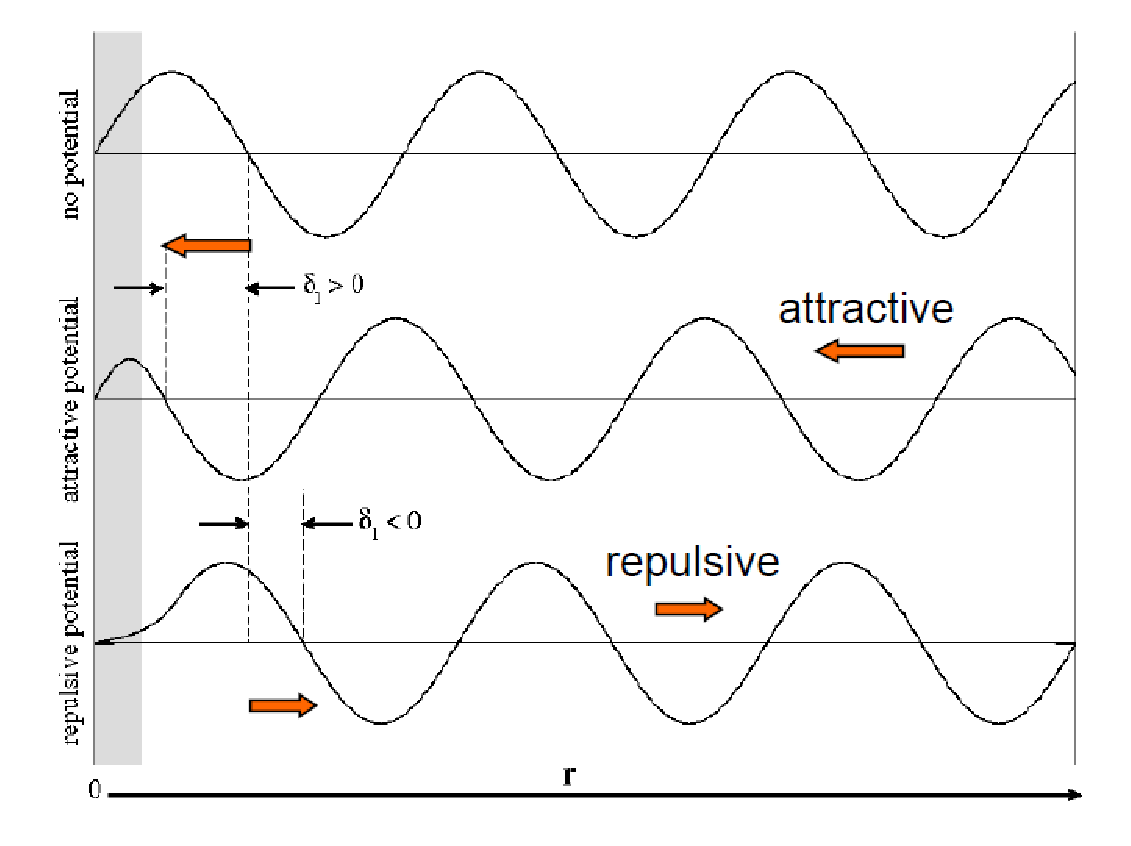
\includegraphics{\images/phaseshifts.eps}} \par}
%\end{figure}
%}%only




\end{frame}




% -------------------------------------------------------------------------
\slide{The scattering amplitude}

\begin{itemize}
\gitem {Replace the asymptotic $\chi_{\ell}(K,R)$ in the general expansion:}

\begin{center}
\psframebox[fillcolor=magenta!5,linecolor=red,framearc=0.1,fillstyle=solid,framesep=-7pt]{
\parbox{0.8\textwidth}{
\begin{align*}
\chi^{(+)}_0 (\bK,\bR) &  \rightarrow  \frac{1}{K R} \sum_{\ell} i^\ell (2 \ell +1)
   {\blue \left \{  F_\ell(K R) +  T_\ell H^{(+)}_\ell (K R)  \right \} }
    P_{\ell}(\cos \theta)   \\
%                         & =  \frac{1}{K R} \sum_{\ell} i^\ell  (2 \ell +1) F_\ell(K R) P_{\ell}(\cos \theta) + 
% \frac{1}{K} \sum_{\ell } i^\ell (2 \ell +1)   T_\ell    \frac{e^{i (K R-\ell \pi/2)}}{R}   P_{\ell}(\cos \theta)  \\
                         & =  e^{i \bK \cdot \bR}  + 
 \frac{1}{K} \sum_{\ell }   (2 \ell +1)  e^{i \delta_\ell} \sin{\delta_\ell}     P_{\ell}(\cos \theta) \frac{e^{i K R}}{R} 
\end{align*}
}%parbox
}%psframe
\end{center}

\gitem{The scattering amplitude is the coefficient of  $e^{i K R}/{R}$:}
\begin{center}
\psframebox[fillcolor=magenta!5,linecolor=red,framearc=0.1,fillstyle=solid,framesep=-7pt]{
\parbox{0.7\textwidth}{
\begin{align*} 
f(\theta)  & = \frac{1}{K} \sum_{\ell} (2 \ell +1)  e^{i \delta_\ell} \sin{\delta_\ell}  P_{\ell}(\cos \theta) 
 \\
          & = \frac{1}{2 i K} \sum_{\ell}(2 \ell +1) (S_\ell -1 ) P_{\ell}(\cos \theta) .
\end{align*} 
}%parbox
}%psframe
\end{center}

\gitem{Elastic cross section:}
$$
\frac{d\sigma}{d\Omega} = | f(\theta) | ^ 2  .
$$ 
\end{itemize}

\end{frame}



% -------------------------------------------------------------------------
\slide{Coulomb plus nuclear case}
{\verde Radial equation:}
\begin{columns}
%\column{0.5\linewidth}
\begin{column}[t]{0.55\textwidth}
$$
\psframebox[fillcolor=magenta!5,linecolor=red,framearc=0.1,framesep=2pt]{
\left [ \frac{d^2}{dR^2} + K^2 - {\blue \frac{2 \eta K}{R}} +
   \frac{2 \mu}{\hbar^2}U(R)+ \frac{\ell (\ell +1)}{R^2} \right ]  \chi_\ell(K, R) = 0
}%psframe
$$
\end{column} %\hfill
\hspace{0.5cm}
\begin{column}[t]{0.4\textwidth}
\vspace{0.4cm}
%\hspace{1.5cm}
%\hfill
$$
\small
\psframebox[linecolor=blue,framearc=0.1,framesep=2pt]{
\eta= \frac{Z_p Z_t e^2}{\hbar v } = \frac{Z_p Z_t e^2 \mu}{\hbar^2 K}
}%psframe
$$
\begin{center}(Sommerfeld parameter) \end{center}
\end{column}
\end{columns}



%\begin{block}{Pure Coulomb wave}
%\end{block}

{\verde Asymptotic condition:}
$$
\chi^{(+)}(\bK,\bR)  \rightarrow e^{i [\bK \cdot \bR +\eta \log (kR-\bK \cdot \bR )]}+ 
                    f(\theta) \frac{e^{i ( KR- \eta \log 2 K R)}}{R}  
$$

%\begin{block}{Asymptotic condition}

\begin{columns}
\column{0.55\columnwidth}
\small
\psframebox[fillcolor=magenta!5,linecolor=red,framearc=0.1,fillstyle=solid,framesep=0pt]{
\parbox{0.95\textwidth}{
\begin{align*}
\chi_\ell (K,R) & \rightarrow {\red e^{i \sigma_\ell}} \left [ F_\ell (\eta,KR) + T_\ell H^{(+)}_\ell (\eta, KR)  \right ]  \\
              & = (i/2) {\red e^{i \sigma_\ell}}\left [  H^{(-)}_\ell  (\eta,KR) -S_\ell H^{(+)}_\ell (\eta, KR)  \right ] 
\end{align*}
}%parbox
}%psframe
\column{0.44\columnwidth}
\small
\ding{43} $\sigma_{\ell} (\eta)$=Coulomb phase shift \\
\ding{43} $F_{\ell} (\eta,KR)$=regular Coulomb wave \\
\ding{43} $H^{(\pm)}_\ell (\eta,KR)$=outgoing/ingoing Coulomb wave
%\end{block}
\end{columns}
\end{frame}








% -------------------------------------------------------------------------
\slide{Coulomb plus nuclear case: scattering amplitude}

Total scattering amplitude:
$$
\psframebox[fillcolor=magenta!5,linecolor=red,framearc=0.1,fillstyle=solid,framesep=7pt]{
f(\theta) = f_C (\theta) + \frac{1}{2 i K} \sum_{\ell} (2 \ell +1) e^{2 i \sigma_\ell} (S_\ell -1) P_\ell(\cos \theta)
}%psframe
$$

\ding{43}
$f_C(\theta)$ is the amplitude for pure Coulomb:

$$
\psframebox[fillcolor=magenta!5,linecolor=red,framearc=0.1,fillstyle=solid,framesep=7pt]{
\frac{d\sigma_R}{d \Omega} = |f_C(\theta)|^2 = \frac{\eta^2}{4 K^2 \sin^4(\frac{1}{2}\theta) } = 
\left ( \frac{Z_p Z_t e^2}{4 E}  \right )^2  \frac{1}{\sin^4(\frac{1}{2}\theta)}
}%psframe
$$

\end{frame}

%-----------------------------------
\slide{Integrated cross sections}

\begin{itemize}
\item Total {\blue elastic} cross section (uncharged particles!)
$$
\psframebox[fillcolor=magenta!5,linecolor=red,framearc=0.1,fillstyle=none,framesep=2pt]{
\sigma_{el} = \int d\Omega \frac{d\sigma}{d\Omega} = \frac{\pi}{K^2} \sum_{\ell} (2 \ell + 1) |1 - S_\ell|^2  
}%
$$
 
\item Total {\blue reaction} cross section (loss of flux from elastic channel) 
$$
\psframebox[fillcolor=magenta!5,linecolor=red,framearc=0.1,fillstyle=none,framesep=2pt]{
\sigma_{reac} = \frac{\pi}{K^2} \sum_{\ell} (2 \ell + 1) (1 - |S_\ell|^2) =\frac{\pi}{K^2} \sum_{\ell} (2 \ell + 1) |T_\ell|^2  
}%
$$


\end{itemize}

\end{frame}







% ----------------------------------------------------------------------------------
\slide{$^4$He+$^{58}$Ni example}


{\brick Effective potential:} $U(R)= U_{nuc}(R) +  U_{coul}(R) $

\begin{figure}{\par \resizebox*{0.5\textwidth}{!}
{\includegraphics{\images/he4ni_veff.eps}} \par}
\end{figure}
\ding{43} The maximum of $V_\mathrm{nuc}(R)+V_C(R)$ defines the Coulomb barrier. Approximately:
$$
\psframebox[fillcolor=magenta!5,linecolor=red,framearc=0.1,fillstyle=none,framesep=2pt]{
R_b \simeq 1.44(A_p^{1/3} + A_t^{1/3})~\textrm{fm}
}%psframe
\quad
\psframebox[fillcolor=magenta!5,linecolor=red,framearc=0.1,fillstyle=none,framesep=2pt]{
 E_b \simeq \frac{Z_p Z_t e^2}{R_b}=\frac{Z_p Z_t}{(A_p^{1/3} + A_t^{1/3})} ~ \textrm{MeV}
}%psframe
$$
\end{frame}
% ----------------------------------------------------------------------------------




% -------------------------------------------------------------------------
\slide{Effect of indicent energy}
%------------------------------------------------------------------------

\ding{43} Depending on the bombarding energy $E$ and the charges of the interacting nuclei, we observe different patterns 
 of elastic scattering. 

\vspace{0.5cm}
\ding{43} For medium/heavy systems, this can be characterized in terms of the Coulomb (or Sommerfeld) parameter: 
{\blue $$\eta = {Z_p Z_t  e^2 \over  4 \pi \epsilon_0 \hbar v}$$ }

%\vspace{0.5cm}
\begin{itemize}
\setlength{\itemsep}{16pt}
\gitem{$E$ well above the Coulomb barrier} {\blue ($\eta \lesssim 1$)} $\Rightarrow$ Fraunhofer scattering
\gitem{$E$ around the Coulomb barrier} {\blue ($\eta \gg 1$)} $\Rightarrow$ Fresnel scattering
\gitem{$E$ well below the Coulomb barrier} {\blue ($\eta \ggg 1$)} $\Rightarrow$ Rutherford scattering 
\end{itemize}

\end{frame}



% ----------------------------------------------------------------------------------
\slide{Elastic scattering: energy dependence}


% --------------- Absolute cross sections --------
\begin{minipage}[t]{.32\textwidth}
\begin{figure}{\par \resizebox*{0.75\textwidth}{!}
{\includegraphics{\images/he4ni_e5_abs.eps}} \par}
\end{figure}
%\center{Rutherford  scattering}
\end{minipage}
% -----------------------------------------------
\begin{minipage}[t]{.32\textwidth}
\begin{figure}{\par \resizebox*{0.75\textwidth}{!}
{\includegraphics{\images/he4ni_e10_abs.eps}} \par}
\end{figure}
%\center{Fresnel}
\end{minipage}
% -----------------------------------------------
\begin{minipage}[t]{.32\textwidth}
\begin{figure}{\par \resizebox*{0.75\textwidth}{!}
{\includegraphics{\images/he4ni_e25_abs.eps}} \par}
\end{figure}
%\center{Fraunh\"ofer}
\end{minipage}
% -----------------------------------------------

\vspace{0.5cm}

% --------------- Relative cross sections ---------------------
\begin{minipage}[t]{.32\textwidth}
\begin{figure}{\par \resizebox*{0.75\textwidth}{!}
{\includegraphics{\images/he4ni_e5.eps}} \par}
\end{figure}
\center{\bf Rutherford  scattering }
\end{minipage}
% -----------------------------------------------
\begin{minipage}[t]{.32\textwidth}
\begin{figure}{\par \resizebox*{0.75\textwidth}{!}
{\includegraphics{\images/he4ni_e10.eps}} \par}
\end{figure}
\center{\bf Fresnel}
\end{minipage}
% -----------------------------------------------
\begin{minipage}[t]{.32\textwidth}
\begin{figure}{\par \resizebox*{0.75\textwidth}{!}
{\includegraphics{\images/he4ni_e25.eps}} \par}
\end{figure}
\center{\bf Fraunh\"ofer}
\end{minipage}
% -----------------------------------------------

\end{frame}
% --------------------------------------------------------------------------------------




% ----------------------------------------------------------------------------------
\slide{Effect of indicent energy (cont.)}

{\bf \brick Example:}  {\bf \nuc{4}{He}+\nuc{58}{Ni} at E=5, 10.7, 25 and 50 MeV} 

\medskip

\ding{43} {\bf Coulomb barrier:} $R_b\simeq 7.8$~fm ; ~~~ $V_b\simeq 10.2$~MeV


\medskip

{\large 
\begin{center}

 \begin{tabular}{|ccccc|}
\hline
 {\blue \bf $E_\mathrm{lab}$ } &  {\blue \bf $\eta$} &  {\blue \bf $ K$ } &  {\blue \bf  $\lambdabar=1/K$}  & {\blue \bf $2 a_0$(*)} \\
(MeV)    &                    &       (fm$^{-1}$)      &  (fm)            & (fm)         \\   
\hline
  5      &      7.95       &         0.920        & 1.087     &      17.2  \\
10.7     &      5.62       &         1.34         & 0.746     &      8.06  \\
25       &      3.55       &         2.06         & 0.485     &      3.44   \\
50       &      2.51       &         2.91         & 0.343     &      1.69  \\
\hline
 \end{tabular}
\end{center}
{\small (*) classical distance of closest approach in head-on collision.}

\bigskip

%\ding{43} ${\blue \eta = {Z_1 Z_2  e^2 \over  4 \pi \epsilon_0 \hbar v} }$

\begin{itemize}
\item {\bf \blue $\eta \ggg 1$}: Rutherford scattering: 
{\verde $\sigma (\theta) \propto 1/\sin^4(\theta/2)$}
\item {\bf \blue $\eta \gg  1$}: Fresnel scattering (rainbow)
\item {\bf \blue $\eta \leq 1$}: Fraunhofer scattering (oscillatory behaviour): 
\end{itemize}


}%large
\end{frame}




% -------------------------------------------------------------------------
\slide{Rutherford scattering}

%{\sc \brick Rutherford scattering}


\begin{columns}
\column{0.5\textwidth}
\begin{figure}{\par \resizebox*{0.8\textwidth}{!}
{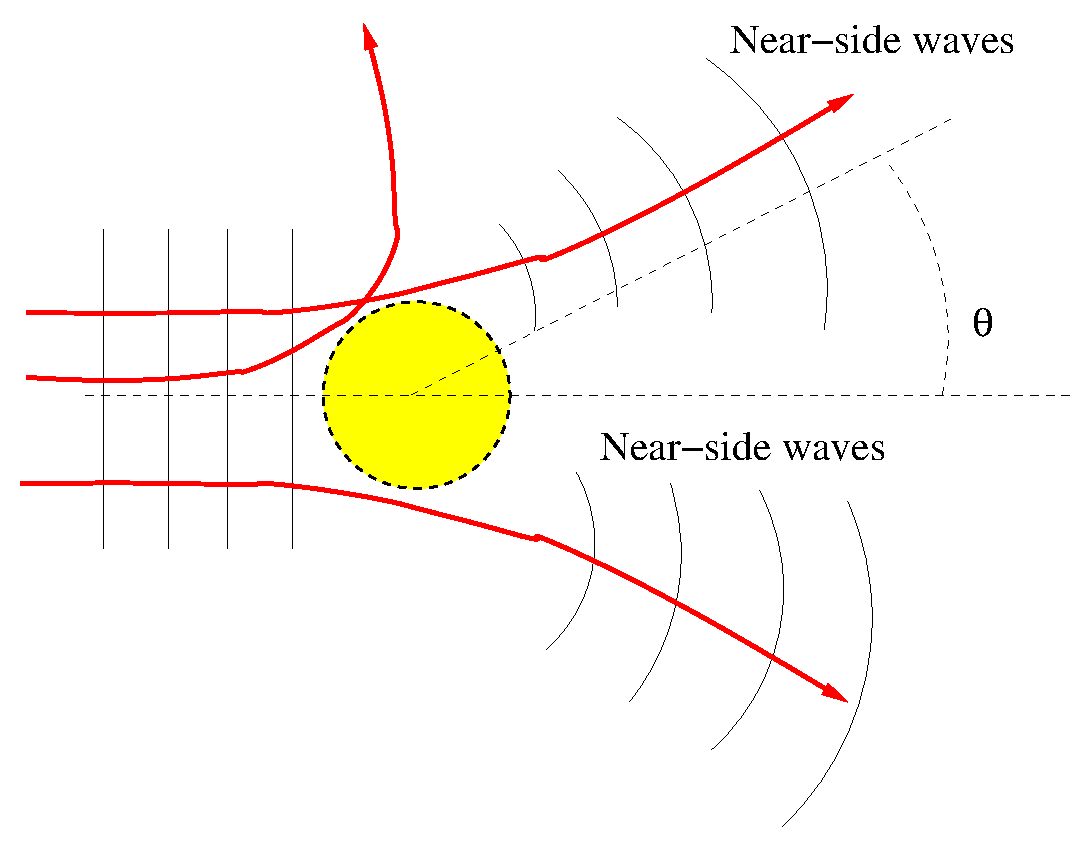
\includegraphics{\images/rutherford.eps}} \par}
\end{figure}
\column{0.5\textwidth}
\begin{figure}{\par \resizebox*{0.65\textwidth}{!}
{\includegraphics{\images/he4ni_e5_abs.eps}} \par}
\end{figure}
\end{columns}


\begin{itemize}
 \item Bombarding energy well below the Coulomb barrier
 \item Purely Coulomb potential ({\verde $\eta \ggg 1$})
 \item Obeys Rutherford law:   
   {\blue $${d \sigma \over d \Omega} = {Z_p Z_t  e^2 \over 4 E} {1 \over \sin^4 (\theta/2)}$$.}
\end{itemize} 

\end{frame}



% -------------------------------------------------------------------------
\slide{Fraunhofer scattering}

%{\sc \brick FRAUNHOFER scattering:}
%\vspace{0.25cm}

\begin{columns}
\column{0.5\textwidth}
\begin{figure}{\par \resizebox*{1.0\textwidth}{!}
{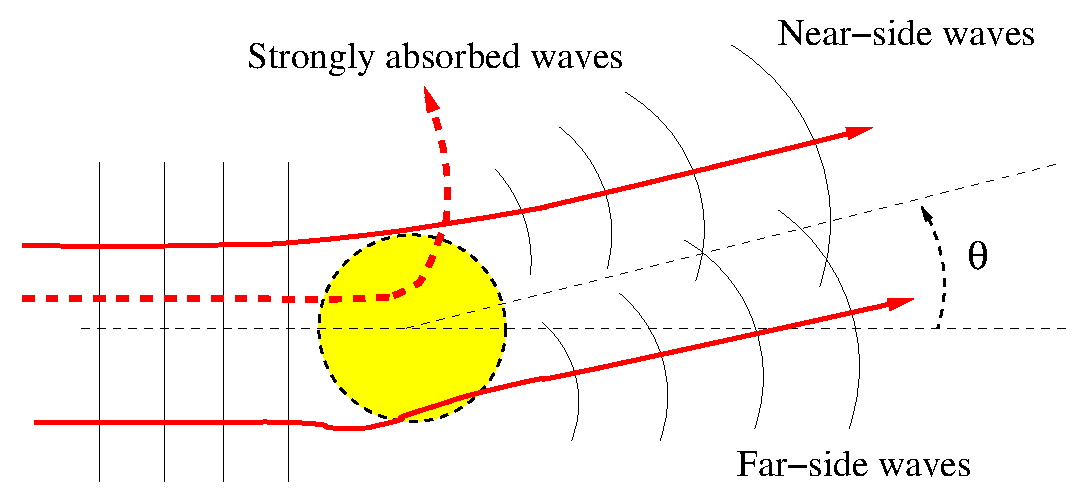
\includegraphics{\images/fraunhofer.eps}} \par}
\end{figure}
\column{0.5\textwidth}
\only<1>{
\begin{figure}{\par \resizebox*{0.65\textwidth}{!}
{\includegraphics{\images/he4ni_e25.eps}} \par}
\end{figure}
}%only
\only<2>{
\begin{figure}{\par \resizebox*{0.65\textwidth}{!}
{\includegraphics{\images/he4ni_e25_nearfa.eps}} \par}
\end{figure}
}%only

\end{columns}

\bigskip

\begin{itemize}
\item Bombarding energy well above Coulomb barrier
\item Coulomb weak ({\verde $\eta \lesssim 1$})
\item Nearside/farside interference pattern  (difracction) 
\end{itemize}

\end{frame}



% -------------------------------------------------------------------------
\slide{Fresnel scattering}

%{\sc \brick FRESNEL scattering:}

%\vspace{0.25cm}


\begin{columns}
\column{0.5\textwidth}
\begin{figure}{\par \resizebox*{0.8\textwidth}{!}
{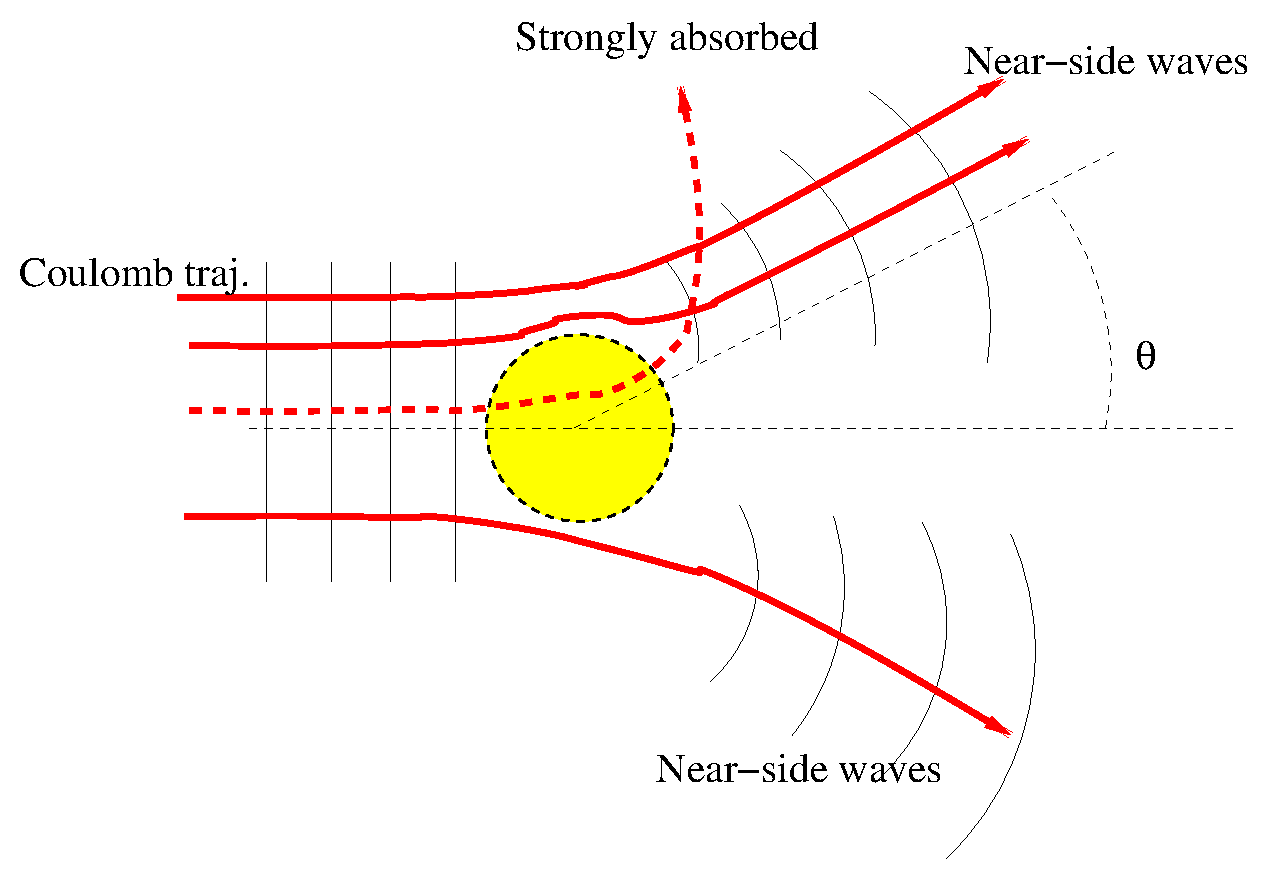
\includegraphics{\images/fresnel.eps}} \par}
\end{figure}
\column{0.5\textwidth}
\begin{figure}{\par \resizebox*{0.65\textwidth}{!}
{\includegraphics{\images/he4ni_e10.eps}} \par}
\end{figure}
\end{columns}


\bigskip

\begin{itemize}
\item Bombarding energy around or near the Coulomb barrier
\item Coulomb strong ({\verde $\eta \gg 1$})
\item  'Illuminated' region $\Rightarrow$ Coulomb + nuclear trajectories
\item[] 'Shadow' region $\Rightarrow$ strong absorption
\end{itemize}

\end{frame}





\subsection{Elastic scattering of weakly-bound nuclei}
% ---------------------------------------------------------------------------------------------------
\slide{Normal versus halo nuclei}

{\verde How does the halo structure affect the elastic scatterig?}
\vspace{0.3cm}


\begin{columns}
\column{0.5\textwidth}
\begin{figure}{\par \resizebox*{0.7\textwidth}{!}
{\includegraphics{\images/he4pb_e22.eps}} \par}
\end{figure}
\column{0.5\textwidth}
\begin{figure}{\par \resizebox*{0.7\textwidth}{!}
{\includegraphics{\images/he6pb_e22.eps}} \par}
\end{figure}
\end{columns}
\bigskip

\begin{small}
\begin{itemize}
\item \nuc{4}{He}+\nuc{208}{Pb} shows typical Fresnel pattern and ``standard'' optical model parameters
%$\rightarrow$ {\blue \em strong absorption} 
\item \nuc{6}{He}+\nuc{208}{Pb} shows a prominent reduction in the elastic cross section, suggesting that part of the incident flux goes to non-elastic channels (eg.~breakup) 
\item[] Understanding and disentangling these non-elastic channels requires going beyond the optical model (eg.~{\blue coupled-channels method} $\Rightarrow$ next lectures) 
\end{itemize}
\end{small}
%}%onslide
\end{frame}


% ------------------------------------------------------------------------------------------------
\slide{Origin of the long-range absorption in $^6$He}

\small
\begin{columns}
\column{0.5\textwidth}

\begin{center}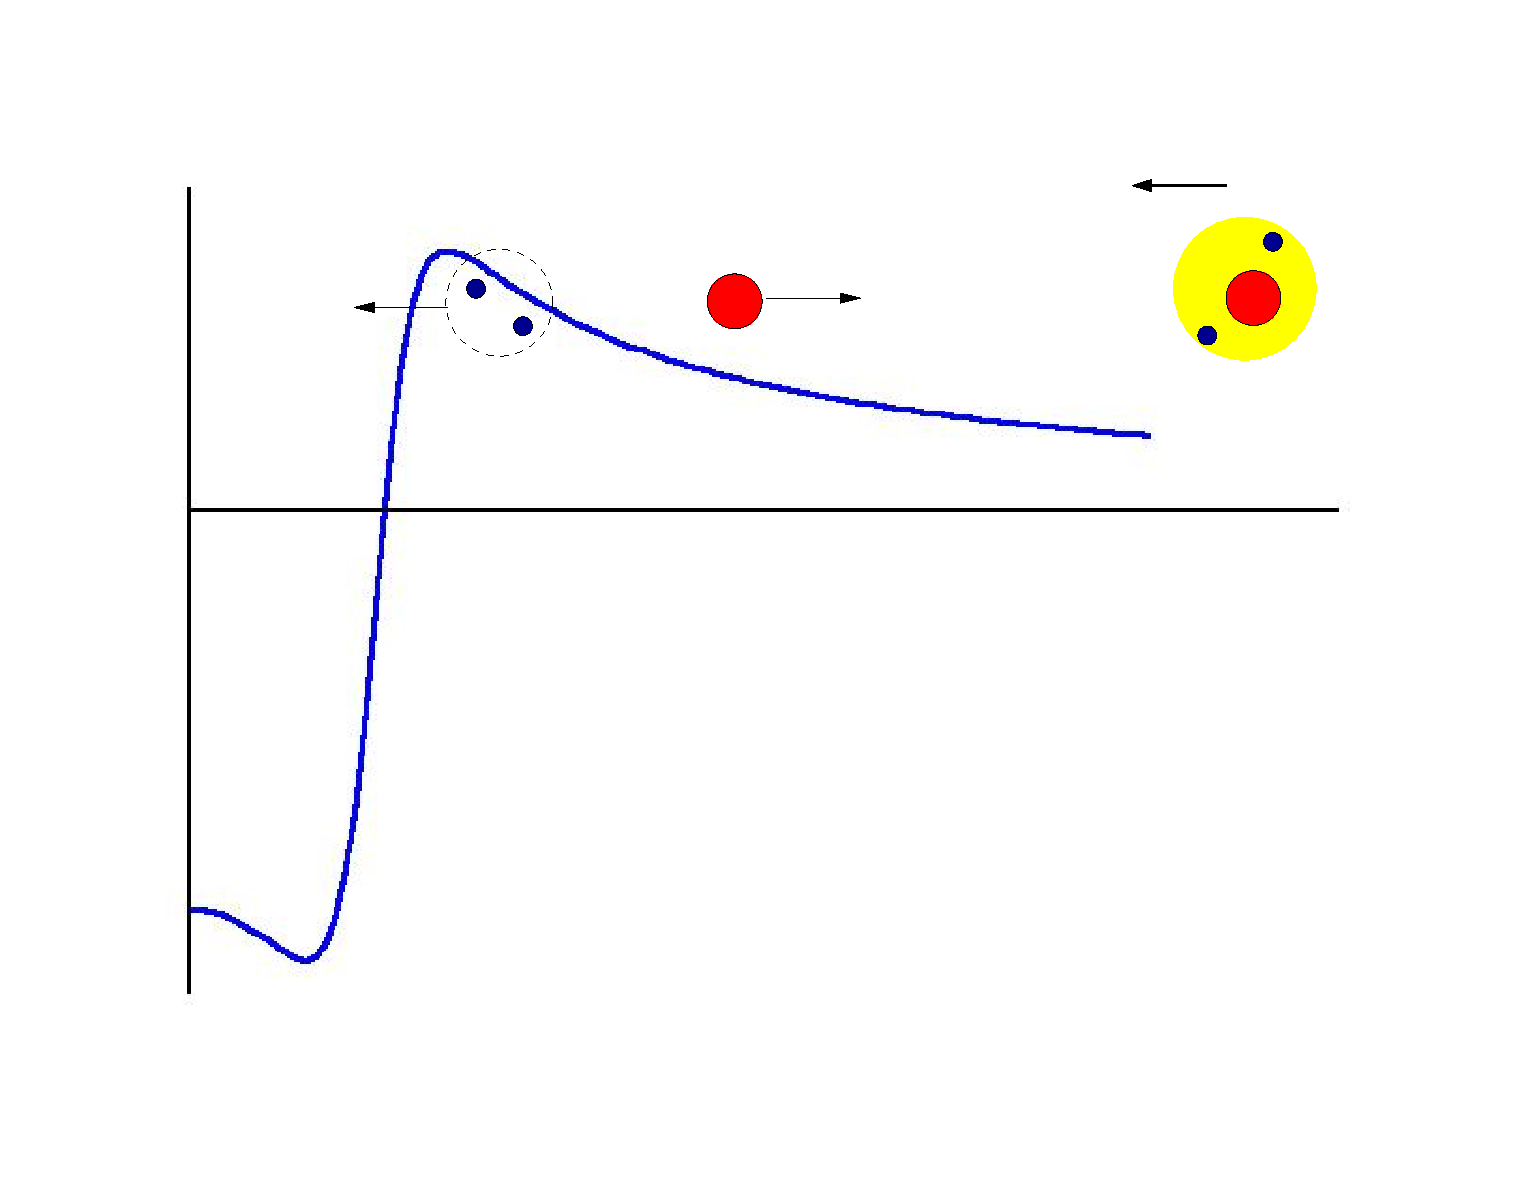
\includegraphics[height=4.5cm]{\images/6he-tidal.eps} \end{center}

\column{0.5\textwidth}
\begin{center}\includegraphics[height=4.5cm]{\images/be1-he6.eps} \end{center}
\end{columns}

\bi
\item[\ding{233}] The Coulomb force on the core induces a tidal force which may eventually break $^{6}$He.
\item[\ding{233}] From the structure point of view, this translates into a large $B(E1)$ strength near breakup threshold.
\ei
\end{frame}




%----------------------------------------------------------
\slide{Second order perturbative amplitude}

\begin{center}
\psframebox[fillcolor=magenta!5,linecolor=red,framearc=0.1,fillstyle=solid,framesep=-8pt]{
\parbox{0.75\textwidth}{
\begin{align*}
c^{(2)}_n = & \sum_{z} \left({-i \over \hbar}\right)^2 
  \int_{-\infty}^{+\infty} dt {\red \langle  n | V_1(t) | z \rangle}
  \exp \left\{ {i \over \hbar}(E_n - E_z) t \right\} \\
 & \times 
  \int_{-\infty}^{t} dt' {\red \langle  z | V_1(t') | 0 \rangle}
  \exp \left\{ {i \over \hbar}(E_z - E_0) t' \right\}
\end{align*}
}%parbox
}%psframe
\end{center}

\begin{center}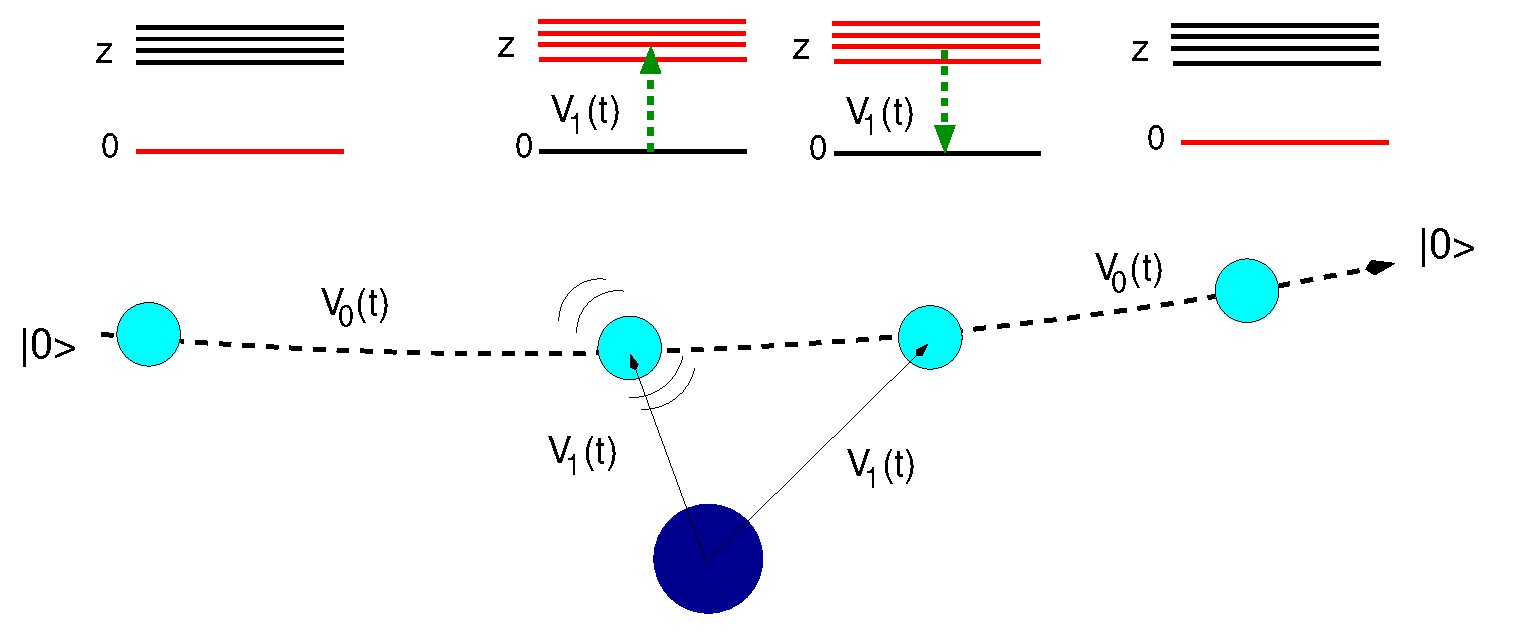
\includegraphics[width=0.8\columnwidth]{\images/a1_traj.eps}  \end{center}

\end{frame}


% --------------------------------------------------------------------------------------
\slide{\small How does a weakly bound nucleus behaves in the field of a heavy target?}

\begin{enumerate}
\item The strong Coulomb field will produce a polarization (``stretching'') of the projectile, giving rise 
to a dipole contribution on the \textcolor{blue}{real} potential:
$$V(R) \approx \frac{Z_1 Z_2 e^2}{R} - \alpha \frac{Z_1 Z_2 e^2}{2 R^4}$$

\item The weakly bound nucleus can eventually break up, leading to a loss of flux of the elastic channel $\Rightarrow$ \textcolor{blue}{imaginary} polarization potential.
\end{enumerate}

\end{frame}



% ---------------------------------------------------------------------------------------------------
\slide{The effect of E1 on elastic scattering of weakly-bound nuclei}

\begin{columns}
\column{0.5\textwidth}
\begin{figure}{\par \resizebox*{0.86\textwidth}{!}
{\includegraphics{\images/he6pb_e22_om.eps}} \par}
\end{figure}
\column{0.5\textwidth}
\begin{figure}{\par \resizebox*{0.7\textwidth}{!}
{\includegraphics{\images/he6pb_cdp.eps}} \par}
\end{figure}
\end{columns}
\bigskip

\begin{small}
\begin{itemize}
\item E1 Coulomb couplings produces a sizable effect on the elastic cross section of neutron-halo nuclei (we have learnt something!) but...some additional physics is still missing. 
\end{itemize}
\end{small}
%}%onslide
\end{frame}




%---------------------------------------------------------------------------------------
\slide{Eg: deuteron polarizability from d+\nuc{208}{Pb}: }

\begin{itemize}
\setlength{\itemsep}{0pt}
%\item[\ding{43}] Deuteron polarizability: $\mathbf{P}= \alpha \mathbf{E}$ 
%\item[\ding{43}] For $E< V_b$,  the main deviation from Rutherford scattering comes from dipole polarizability. 
\item[\ding{43}] Adiabatic limit ($E_x \gg$ ): $V_\mathrm{pol}^\mathrm{dip}=- \alpha \frac{Z_1 Z_2 e^2}{2 R^4}$
\end{itemize}

%\psshadowbox[fillcolor=lightgreen]{{\sc \brick Radius of sensitivity of V(r) and W(r)}}

\begin{columns}[c]
\column{.5\textwidth}
\begin{figure}{\par \resizebox*{0.75\textwidth}{!}
{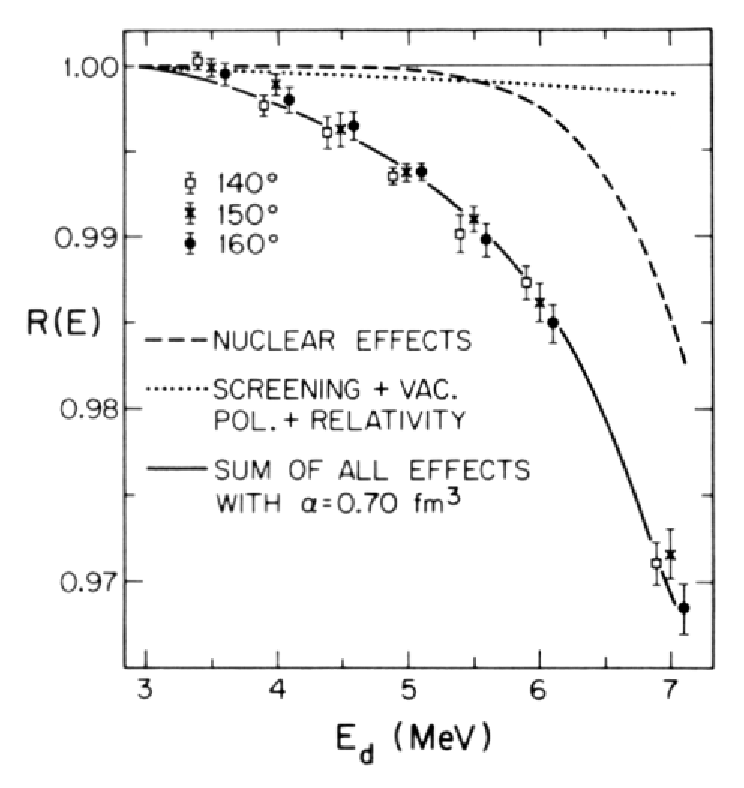
\includegraphics{\images/RE.eps}} \par}
\end{figure}
\column{.5\textwidth}
\begin{figure}{\par \resizebox*{0.75\textwidth}{!}
{\includegraphics{\images/dpb_scattering.eps}} \par}
\end{figure}
\end{columns}%twocolumn
\medskip
\small 
\textcolor{verde}{\small Rodning et al, PRL49, 909 (1982)} $\Rightarrow$ \textcolor{red}{$\alpha = 0.70 \pm 0.05 $~fm$^3$}

\end{frame}

\endinput

%%%%%%%%%%%%%%%%%%%%%%
% BACKUP SLIDES FOR ELASTICS
%%%%%%%%%%%%%%%%%%%%%%
\slide{}
\begin{center}
\psframebox[fillcolor=green!10,linecolor=blue,framearc=0.1,fillstyle=solid,framesep=5pt]{
SUPPLEMENTARY MATERIAL
}%psframe
\end{center} 
\end{frame}





% ---------------------------------------------------------------------------
\slide{Grazing radius and angular momentum}

\begin{itemize}
\setlength{\itemsep}{14pt}
\item Grazing collisions are those for which $b \approx R_1 + R_2 = R_g$ 

\item Relation with angular momentum:
\begin{enumerate}
\item {\blue Only nuclear:} $b K = \sqrt{\ell (\ell +1) } \simeq \ell +1/2$
$$
\psframebox[fillcolor=magenta!5,fillstyle=solid,linecolor=red,framearc=0.1]{
K R_g \simeq \ell_g +1/2
}
 \quad (\ell_g=\textrm{grazing angular momentum})
$$
\item {\blue Nuclear + Coulomb:}
$$
\psframebox[fillcolor=magenta!5,fillstyle=solid,linecolor=red,framearc=0.1]{
K R_g \left(1- 2 \eta /K R_g  \right)\approx \ell_g +1/2 
}%
$$
\end{enumerate}

\item[\ding{233}] As $E$ increases, so does the number of partial waves involved
\item[\ding{233}] Peripherical processes (inelastic, transfer) occur mainly around $\ell \sim \ell_g$
\end{itemize}

\end{frame}




% ----------------------------------------------------------------------------------
\slide{Elastic scattering: S-matrix elements}

{\brick Elastic (nuclear) S-matrix :} $\chi_{\ell}(K,R) =H^{(-)}_{\ell}(R) -  S_\ell H^{(+)}_\ell(R)$


\vspace{0.5cm}

\begin{columns}
\column{0.5\textwidth}
\begin{figure}{\par \resizebox*{0.95\textwidth}{!}
{\includegraphics{\images/4he58ni_smat.eps}} \par}
\end{figure}
\column{0.5\textwidth}
\begin{figure}{\par \resizebox*{0.95\textwidth}{!}
{\includegraphics{\images/4he58ni_reac.eps}} \par}
\end{figure}
\end{columns}

\medskip

\begin{center}
{\blue  $K R_g \left(1- 2 \eta /K R_g  \right)\approx \ell_g +1/2$} 
\end{center}


$\Rightarrow$ the number of partial waves 
required for convergence grows approximately as $\sqrt{E}$ 


\end{frame}

\endinput

% --------------------------------------------------------------------------
\slide{Elastic scattering phenomenology }


{\bf \verde What can we learn from the  analysis of the elastic cross section?}

\vspace{1cm}

% --------------- Absolute cross sections --------
\begin{minipage}[t]{.32\textwidth}
\begin{figure}{\par \resizebox*{0.84\textwidth}{!}
{\includegraphics{\images/dni_e80_el_dat.eps}} \par}
\end{figure}
%\center{Rutherford  scattering}
\end{minipage}
% -----------------------------------------------
\begin{minipage}[t]{.32\textwidth}
\begin{figure}{\par \resizebox*{0.84\textwidth}{!}
{\includegraphics{\images/he4pb_e22_exp.eps}} \par}
\end{figure}
%\center{Fresnel}
\end{minipage}
% -----------------------------------------------
\begin{minipage}[t]{.32\textwidth}
\begin{figure}{\par \resizebox*{0.84\textwidth}{!}
{\includegraphics{\images/he6pb_e22_data.eps}} \par}
\end{figure}
%\center{Fraunh\"ofer}
\end{minipage}
% -----------------------------------------------

\bigskip

\end{frame}





